\chapter{Background}
\label{cha:background}

In this section, there will be all the background information relevat to the thesis,
that are needed in order to properly understand the matter of the project, the problem,
the technologies and the solution.

We will start in subsection \ref{cha:CPU speculation contract} by explaining
what a CPU speculation contract is, and why it is important for the scope of this
thesis. Then we will move to subsection \ref{cha:Revizor}, where we will talk about
the Revizor tool, that is used in the project to detect the contract of a CPU. We
will detail how it works and some background information. In subsection
\ref{cha:Rosette}, we will talk about Rosette, the solver-aided programming
language that is used to encode the violations reported from Revizor. In subsection
\ref{cha: Loop outlook}, we will give an overview of the loop that is used to
synthesize the CPU contract, using all the tools anbd language discussed in previous
sections. In subsection \ref{cha:DSL}, we will talk about the Domain Specific Language
(DSL) that the team used before this thesis's project, and why it was not enough
for the scope of the overall project. In subsection \ref{cha:BIR}, we will talk
about the Binary Intermediate Representation (BIR) language, that has been chosen
to replace the DSL, and why it is a better choice for the project.

\section{CPU speculation contract}
\label{cha:CPU speculation contract} Before diving into what a CPU speculation
contract is, it is better to have a clear idea of what speculative execution is.
In speculative exection, the CPU tries to predict the path of a branch operation
before the actual path is known. This is done to increase performance, as the CPU
can execute instructions beforehand. Once the actual path is known, the CPU can discard
or confirm the speculative execution.

\begin{figure}
  \centering
  \begin{varwidth}
    {\linewidth} \begin{verbatim}
      if (x == 1) {
        y = 1;
      } else {
        y = 2;
      }
          \end{verbatim}
  \end{varwidth}
  \label{fig:snip1}
  \caption{Conditional statement}
\end{figure}

For example, consider the snipper in \ref{fig:snip1}. The CPU can predict that
the path will be the one on the true branch (hence, `y=1`), and evaluate it. At this
point, the CPU has to check if the condition holds, evaluating the predicate. If
the evaluation confirms that the speculation was right, the CPU can confirm the speculative
execution, and continue with the exection. Otherwise, it will discard the
execution and run the real path.

Whis this in mind, the speculation contract of a CPU can be seen as an agreement
or policy that governs the behaviour of the speculative execution. A contract is
usually formed by different so-called constraints, that are all the rules that the
CPU has to follow in order to be compliant with the contract. All constrains are
usually encoded with the machine specific code of the CPU, that is not accessible
from the users. This is why we ofter refer to this contract as a black-box
contract.

One of the main goals of this project is synthesizing this contract, using all the
tools that will follow in the next sections, and then represent them in a human-readable,
standard language. This language, at the beginning was a DSL (\ref{cha:DSL}),
but in this thesis project, I replaced it with BIR (\ref{cha:BIR}).

\section{Revizor}
\label{cha:Revizor} Revizor is an open source fuzzing tool developed by a Microsoft
Research team \cite{article}. It has been developed to detect black-box CPU
informational leakeages, just starting from a CPU speculation contract (\ref{cha:CPU
speculation contract}). Then, it generates a number of test cases, executing
therefore some fuzzing to detect evantual leakeages in the contract. Once the test
cases has been generated, they are runned on the CPU, and then Revizor looks at the
information that are leaked, and then compare them with the CPU contract. With this
information, we are able to understand if the CPU is leaking information.

The researchers tested Revizor on different x86 Intel CPUs, finding some known vulnerabilities,
such as Spectre, MDS (Microarchitectural Data Sampling) and LVI (Load value
injection), and some novel ones. All this is done in a short amount of time, in
an automated fashion. The tool is mainly written in Python, with some C code for
performance improvements. It is available on GitHub (\cite{repo}), and can be
used by anyone to test any CPU. The documentation of Revizor is full of examples
and tests made (\cite{misc}).

In this project, Revizor is used as part of the toolchain, to detect the contract
of a CPU. starting from our current CPU leakeage contract, we run Revizor on this
specification, and then we check if we obtain some violations. If so, we add the
discovered violations to the contract, enriching it with novel information about
the CPU. And then we loop over. The loop will be futher discussed in Section \ref{cha:
Loop outlook}.

\section{Rosette}
\label{cha:Rosette} Rosette is an open-source solver-aided programming language.
It is Racket-based and allows to write programs that are able to generate and
solve constraints. So, it takes care of verifying and syntehtizing programs, making
easier to build Domain Specific Languages, and does the heavy lifting on its own,
making easier for the user to write the code.

In the project, Rosette is used to encode the violations reported from Revizor (\ref{cha:Revizor})
into new constrains for the CPU contract. This continue iterating in the loop until
the contract is stable. It has been chosen as it makes the development of the
tools needed to handle, verify and synthesise the contracts easier, faster and
more reliable. Also, Rosette is one of the most used and known tools in this
field, so it is well documented, and futher and future development can be done
by other members of the research community.

\section{Loop outlook}
\label{cha: Loop outlook} The project works by iterating a loop for syntehtizing
the CPU contract. Here is a brief overview of the loop. At the end of the
section, there is also a flowchart that should give a more visual and intuitive grasp
of the matter of it.

We start with a CPU with an initial contract, being empty. At this point, we
pass it through Revizor, that will generate the test cases and will run them on the
CPU. Once done, Revizor will check if there are any violations, and in case will
return them. At this point, we generate this violations, and using Rosette, we
generate new constraints to add in the CPU contract. Once the contract has been updated,
we can start to loop again with Revizor and Rosette, unitl we reach a stable contract,
our aimed fixed point.

This final fixed point, will be the syntesized CPU contract, that we are sure is
correct and complete for our specific CPU. This will be the final output of the toolchain.
\begin{center}
  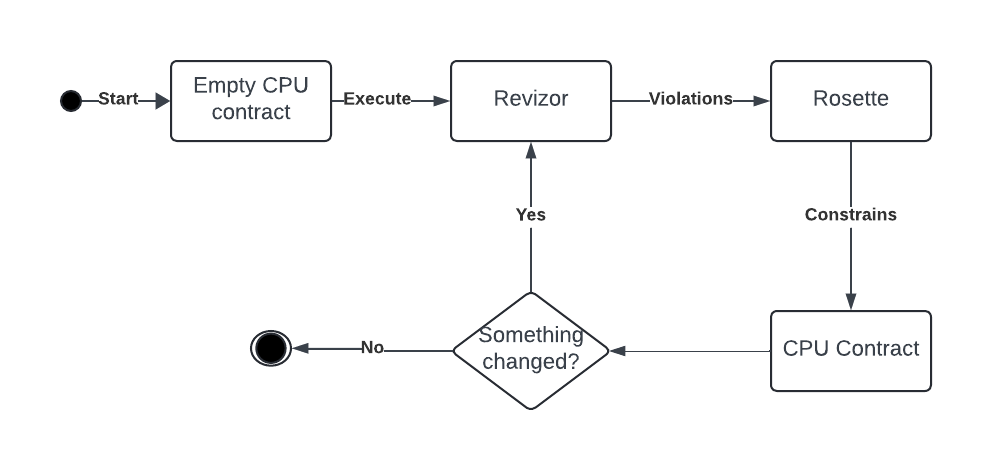
\includegraphics[width=.6\textwidth]{images/Thesis.png}
\end{center}

\section{DSL}
\label{cha:DSL} To represent the CPU contract, we needed a language that was
able to describe the ISA of a CPU and its contract. To archieve this need, at
the beginning of the project, a Domain Specific Language (DSL) was developed.
This language is able to define, check and evaluate a number of boolean conditions,
such as AND, OR, NOT, EQUAL, and to access CPU's registers. This was enough as a
proof of concept to see wheather the whole system was working, but now with the
further steps of the project, this is not enough anymore. To have a more
research-validated, robust, complete and universal language, the team decided to
switch from this DSL to using the BIR language (more in Section \ref{cha:BIR}).

\section{BIR}
\label{cha:BIR} Binary Intermediate Representation (BIR) is a programming language
developed by a group of researchers, that were trying to make analysis of binary
files. To do so, they needed a language that was platform independent, and that represented
the ISA of a CPU. The goal of the language is to be clear, meaning that it has only
explicit type changes, leaving no room for side effects and abstracted
behaviours. BIR has functionalities such as blocks, jump, assignent and so on.
In our project, the part of BIR that was used are the expressions. When we talk
about expressions in BIR we mean the following possible statements:
\begin{itemize}
  \item \textbf{Constant}: A constant value, in our case a numeric value.

  \item \textbf{Unary operation}: Operation performed on a singular value, such
    as binary NOT.

  \item \textbf{Binary expressions }: A function that can be called with a number
    of arguments.

  \item \textbf{Binary operation}: Operation performed on two values, such as
    binary AND.

  \item \textbf{Predicates}: A function that returns a boolean value.

  \item \textbf{Variable}: Usage of variables, such as the value inside a given
    register.

  \item \textbf{IfThenElse statement}: A conditional statement with a condition,
    and two branches that are evaluated according to the condition itself.

  \item \textbf{Load}: Load a value from a given memory address.

  \item \textbf{Store}: Store a value in a given memory address.
\end{itemize}

Followig there is a simple example of each one of the possible expressions that
has been used in the project, with a brief comment on the meaning of them.
\begin{verbatim}
- (BExp_Const (bv 1 Bit32)) # Constant value 1, in binary vector of 32 bits.
- (BExp_UnaryExp (BIExp_ChangeSign (BExp_Const (bv 42 Bit8)))) # Change sign of 42
- (BExp_BinExp BIExp_Plus (BExp_Const (bv 12 Bit8)) (BExp_Const (bv 30 Bit8))) # Sum
of 12 and 30
- (BExp_BinPred BIExp_Equal (BExp_Const (bv 12 Bit8)) 
(BExp_Const (bv 30 Bit8))) # Check if 12 is equal to 30
- (BExp_Den (BVar R1)) # Value inside register R1
- (BExp_IfThenElse (BExp_BinPred BIExp_Equal (BExp_Const (bv 12 Bit8)) 
(BExp_Const (bv 30 Bit8))) (BExp_Const (bv 42 Bit8)) (BExp_Const (bv 50 Bit8))) 
# If 12 is equal to 30, return 42, else return 50
- (BExp_Load BExp_Den (BVar R1) (BExp_Const (bv 0 Bit32)) BEnd_LittleEndian Bit64) 
# Load value from memory address 0 in R1, in little endian, 64 bits
- (BExp_Store BExp_Den (BVar  R1) (BExp_Const (bv 0 Bit32)) BEnd_LittleEndian 
(BExp_Const(bv 2 Bit32))) # Store value 2 in memory address 0 in R1, in little endian
\end{verbatim}

We choose to substitute the DSL with BIR as it is more robust, complete, platform
independent and research-based. It is also pretty close to multiple different
dilects present in other popular tools such as Valgrind IR. This would make the project
also more usable and extendable in the future, by other actors outside the team
of research.